\chapter[Title in the table of content]{This is a very Long Title This is a very Long Title This is a very Long Title This is a very Long Title}\label{chap:ex}

\section{Long Caption}
Same as the float:
\begin{table}[ht]
\centering
\caption[Ablation study on learning rate]{Ablation study on $\alpha$. Ablation study on $\alpha$. Ablation study on $\alpha$. Ablation study on $\alpha$. Ablation study on $\alpha$. Ablation study on $\alpha$. Ablation study on $\alpha$. Ablation study on $\alpha$. }
\resizebox{\textwidth}{!}{
\begin{tabular}{cccccccccccc}
\hline
\multirow{2}{*}{prompt}                  & \multirow{2}{*}{$\alpha$} & \multicolumn{2}{c}{PSNR$\uparrow$}                                        & \multicolumn{2}{c}{FID$\downarrow$}                                         & \multicolumn{2}{c}{SSIM$\uparrow$}                                          & \multicolumn{2}{c}{LPIPS$\downarrow$}                                       & \multicolumn{2}{c}{ACDM$\downarrow$}                   \\
                                         &                           & SD14                                & SD15                                & SD14                                 & SD15                                 & SD14                                 & SD15                                 & SD14                                 & SD15                                 & SD14                                 & SD15            \\ \hline
\multicolumn{1}{c|}{\multirow{3}{*}{P1}} & \multicolumn{1}{c|}{1}    & \multicolumn{1}{c|}{18.18}          & \multicolumn{1}{c|}{18.18}          & \multicolumn{1}{c|}{137.44}          & \multicolumn{1}{c|}{134.12}          & \multicolumn{1}{c|}{0.4563}          & \multicolumn{1}{c|}{0.4576}          & \multicolumn{1}{c|}{0.6137}          & \multicolumn{1}{c|}{0.6119}          & \multicolumn{1}{c|}{0.1075}          & 0.1080          \\
\multicolumn{1}{c|}{}                    & \multicolumn{1}{c|}{2}    & \multicolumn{1}{c|}{\textbf{18.02}} & \multicolumn{1}{c|}{\textbf{18.02}} & \multicolumn{1}{c|}{\textbf{139.11}} & \multicolumn{1}{c|}{\textbf{135.32}} & \multicolumn{1}{c|}{0.4441}          & \multicolumn{1}{c|}{0.4453}          & \multicolumn{1}{c|}{\textbf{0.6188}} & \multicolumn{1}{c|}{\textbf{0.6171}} & \multicolumn{1}{c|}{\textbf{0.1106}} & \textbf{0.1110} \\
\multicolumn{1}{c|}{}                    & \multicolumn{1}{c|}{4}    & \multicolumn{1}{c|}{18.43}          & \multicolumn{1}{c|}{18.44}          & \multicolumn{1}{c|}{132.79}          & \multicolumn{1}{c|}{132.77}          & \multicolumn{1}{c|}{\textbf{0.4408}} & \multicolumn{1}{c|}{\textbf{0.4419}} & \multicolumn{1}{c|}{0.6057}          & \multicolumn{1}{c|}{0.6049}          & \multicolumn{1}{c|}{0.0961}          & 0.0966          \\ \hline
\multicolumn{1}{c|}{\multirow{3}{*}{P2}} & \multicolumn{1}{c|}{1}    & \multicolumn{1}{c|}{16.85}          & \multicolumn{1}{c|}{16.82}          & \multicolumn{1}{c|}{70.40}           & \multicolumn{1}{c|}{68.52}           & \multicolumn{1}{c|}{0.4448}          & \multicolumn{1}{c|}{0.4445}          & \multicolumn{1}{c|}{0.5956}          & \multicolumn{1}{c|}{0.5938}          & \multicolumn{1}{c|}{0.1131}          & 0.1142          \\
\multicolumn{1}{c|}{}                    & \multicolumn{1}{c|}{2}    & \multicolumn{1}{c|}{\textbf{16.74}} & \multicolumn{1}{c|}{\textbf{16.70}} & \multicolumn{1}{c|}{\textbf{70.59}}  & \multicolumn{1}{c|}{\textbf{69.04}}  & \multicolumn{1}{c|}{0.4336}          & \multicolumn{1}{c|}{0.4329}          & \multicolumn{1}{c|}{\textbf{0.6005}} & \multicolumn{1}{c|}{\textbf{0.5990}} & \multicolumn{1}{c|}{\textbf{0.1156}} & \textbf{0.1167} \\
\multicolumn{1}{c|}{}                    & \multicolumn{1}{c|}{4}    & \multicolumn{1}{c|}{17.10}          & \multicolumn{1}{c|}{17.08}          & \multicolumn{1}{c|}{66.88}           & \multicolumn{1}{c|}{65.54}           & \multicolumn{1}{c|}{\textbf{0.4330}} & \multicolumn{1}{c|}{\textbf{0.4327}} & \multicolumn{1}{c|}{0.5887}          & \multicolumn{1}{c|}{0.5863}          & \multicolumn{1}{c|}{0.1018}          & 0.1026          \\ \hline
\multicolumn{1}{c|}{\multirow{3}{*}{P3}} & \multicolumn{1}{c|}{1}    & \multicolumn{1}{c|}{16.86}          & \multicolumn{1}{c|}{16.91}          & \multicolumn{1}{c|}{155.70}          & \multicolumn{1}{c|}{152.69}          & \multicolumn{1}{c|}{0.4330}          & \multicolumn{1}{c|}{0.4323}          & \multicolumn{1}{c|}{0.6165}          & \multicolumn{1}{c|}{0.6171}          & \multicolumn{1}{c|}{0.1052}          & 0.1053          \\
\multicolumn{1}{c|}{}                    & \multicolumn{1}{c|}{2}    & \multicolumn{1}{c|}{\textbf{16.71}} & \multicolumn{1}{c|}{\textbf{16.78}} & \multicolumn{1}{c|}{\textbf{156.47}} & \multicolumn{1}{c|}{\textbf{153.85}} & \multicolumn{1}{c|}{0.4234}          & \multicolumn{1}{c|}{0.4228}          & \multicolumn{1}{c|}{\textbf{0.6202}} & \multicolumn{1}{c|}{\textbf{0.6204}} & \multicolumn{1}{c|}{\textbf{0.1084}} & \textbf{0.1079} \\
\multicolumn{1}{c|}{}                    & \multicolumn{1}{c|}{4}    & \multicolumn{1}{c|}{17.00}          & \multicolumn{1}{c|}{17.04}          & \multicolumn{1}{c|}{140.65}          & \multicolumn{1}{c|}{139.28}          & \multicolumn{1}{c|}{\textbf{0.4198}} & \multicolumn{1}{c|}{\textbf{0.4189}} & \multicolumn{1}{c|}{0.6110}          & \multicolumn{1}{c|}{0.6108}          & \multicolumn{1}{c|}{0.0958}          & 0.0956          \\ \hline
\multicolumn{1}{c|}{\multirow{3}{*}{P4}} & \multicolumn{1}{c|}{1}    & \multicolumn{1}{c|}{17.75}          & \multicolumn{1}{c|}{17.62}          & \multicolumn{1}{c|}{\textbf{118.34}} & \multicolumn{1}{c|}{113.48}          & \multicolumn{1}{c|}{0.4138}          & \multicolumn{1}{c|}{0.4067}          & \multicolumn{1}{c|}{0.6305}          & \multicolumn{1}{c|}{0.6337}          & \multicolumn{1}{c|}{0.1021}          & 0.1036          \\
\multicolumn{1}{c|}{}                    & \multicolumn{1}{c|}{2}    & \multicolumn{1}{c|}{\textbf{17.61}} & \multicolumn{1}{c|}{\textbf{17.50}} & \multicolumn{1}{c|}{116.48}          & \multicolumn{1}{c|}{\textbf{115.41}} & \multicolumn{1}{c|}{0.4004}          & \multicolumn{1}{c|}{0.3942}          & \multicolumn{1}{c|}{\textbf{0.6361}} & \multicolumn{1}{c|}{\textbf{0.6394}} & \multicolumn{1}{c|}{\textbf{0.1051}} & \textbf{0.1067} \\
\multicolumn{1}{c|}{}                    & \multicolumn{1}{c|}{4}    & \multicolumn{1}{c|}{17.96}          & \multicolumn{1}{c|}{17.85}          & \multicolumn{1}{c|}{110.58}          & \multicolumn{1}{c|}{109.59}          & \multicolumn{1}{c|}{\textbf{0.3929}} & \multicolumn{1}{c|}{\textbf{0.3876}} & \multicolumn{1}{c|}{0.6302}          & \multicolumn{1}{c|}{0.6347}          & \multicolumn{1}{c|}{0.0918}          & 0.0927          \\ \hline
\multicolumn{1}{c|}{\multirow{3}{*}{P5}} & \multicolumn{1}{c|}{1}    & \multicolumn{1}{c|}{16.91}          & \multicolumn{1}{c|}{17.06}          & \multicolumn{1}{c|}{132.37}          & \multicolumn{1}{c|}{128.71}          & \multicolumn{1}{c|}{0.4670}          & \multicolumn{1}{c|}{0.4628}          & \multicolumn{1}{c|}{0.5989}          & \multicolumn{1}{c|}{0.6004}          & \multicolumn{1}{c|}{0.1207}          & 0.1182          \\
\multicolumn{1}{c|}{}                    & \multicolumn{1}{c|}{2}    & \multicolumn{1}{c|}{\textbf{16.81}} & \multicolumn{1}{c|}{\textbf{16.95}} & \multicolumn{1}{c|}{\textbf{134.71}} & \multicolumn{1}{c|}{\textbf{129.93}} & \multicolumn{1}{c|}{0.4568}          & \multicolumn{1}{c|}{0.4524}          & \multicolumn{1}{c|}{\textbf{0.6032}} & \multicolumn{1}{c|}{\textbf{0.6047}} & \multicolumn{1}{c|}{\textbf{0.1227}} & \textbf{0.1209} \\
\multicolumn{1}{c|}{}                    & \multicolumn{1}{c|}{4}    & \multicolumn{1}{c|}{17.18}          & \multicolumn{1}{c|}{17.33}          & \multicolumn{1}{c|}{126.82}          & \multicolumn{1}{c|}{124.19}          & \multicolumn{1}{c|}{\textbf{0.4547}} & \multicolumn{1}{c|}{\textbf{0.4516}} & \multicolumn{1}{c|}{0.5932}          & \multicolumn{1}{c|}{0.5939}          & \multicolumn{1}{c|}{0.1088}          & 0.1073          \\ \hline
\end{tabular}
}
\label{tab:ablation:alpha}
\end{table}

\newpage
\section{Math Formula \texorpdfstring{$\frac{1}{2} \alpha$}{1/2 alpha} Support in the Section Title}\label{math:in:title}
\verb|\|texorpdfstring\{formula\}\{corresponding pure text\}

\section{Citation}
Only support something like Some researchers~\cite{ho2020ddpm} $\cdots$, do not support \verb|\|citeauthor or \verb|\|citeyear.

\section{Draw Figures}
You may need to have some figures in one pdf (for faster compile), here I provide a example how I make it in \boxed{chap-example/figs/draw-figure.tex}. Please note that, you may be unable to compile if you compile the thesis before, just clean the cache or recompile from scratch. Then download it and insert it in the thesis:

\begin{figure}[htbp]
    \centering
    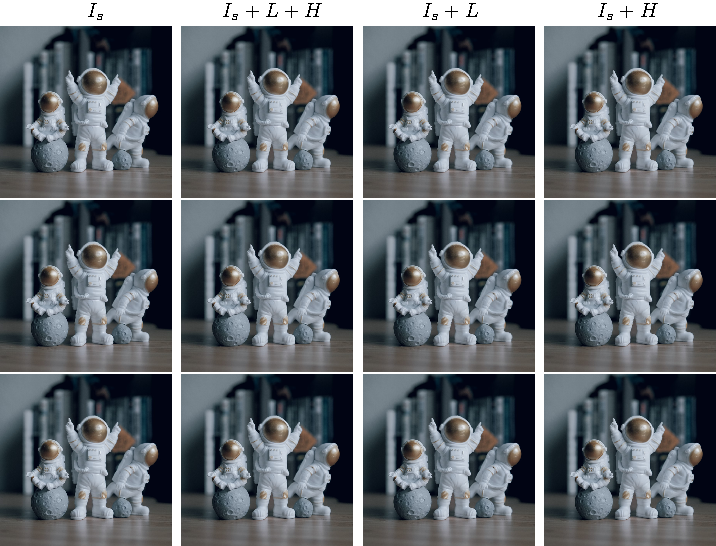
\includegraphics[width=0.6\linewidth]{chap-example/figs/example-fig.pdf}
    \caption[a figure]{long caption. long caption. long caption. long caption. long caption. long caption. long caption. long caption.}
    \label{fig:eg}
\end{figure}

\subsection{Position of the figure}
In line 17, you may notice the htbp. h=here, t=top, b=bottom, p=anywhere of the page. In some case ``h'' doesn't work, try only ``H''.

\section{Useful Tools}
\begin{itemize}
    \item Table: \url{https://tablesgenerator.com/latex_tables}
    \item Formula:
    \url{https://www.latexlive.com/}
    \item Crop pdf's blank border (Usually works for ppt made pdf): \url{https://croppdf.com/}
\end{itemize}